\documentclass[conference, a4paper]{IEEEtran}

\usepackage{amsmath, amssymb, amsthm}
\usepackage{graphicx}
\usepackage{hyperref}
\usepackage{listings}
\usepackage{xcolor}
\usepackage{inconsolata}
\usepackage{booktabs}
\usepackage{siunitx}
\usepackage{microtype}
\usepackage{tikz}
\usetikzlibrary{arrows.meta, positioning, calc, fit, backgrounds, decorations.pathreplacing}

% Warning triangle icon used in the vulnerabilities discussion.
\DeclareRobustCommand{\warnicon}{%
  \tikz[baseline=-0.55ex]{%
    \draw[fill=yellow!85, draw=black, very thick, line join=round]
      (0,0) -- (0.9,1.5) -- (1.8,0) -- cycle;
    \draw[very thick] (0.9,1.05) -- (0.9,0.45);
    \fill (0.9,0.16) circle (0.09);}}

% ------------------------------------------------------------------
% Rust syntax highlighting
% ------------------------------------------------------------------
\lstdefinelanguage{Rust}{
  keywords={as, async, await, break, const, continue, crate, do, dyn, else, enum, extern, false, fn, for, if, impl, in, let, loop, match, mod, move, mut, pub, ref, return, self, Self, static, struct, super, trait, true, type, unsafe, use, where, while, yield},
  keywordstyle=\color{blue}\bfseries,
  ndkeywords={Option, Some, None, Result, Ok, Err, Vec, String, Box, Fn, FnMut, FnOnce, f32, u8, bool},
  ndkeywordstyle=\color{purple}\bfseries,
  comment=[l]{//},
  morecomment=[s]{/*}{*/},
  commentstyle=\color{green!50!black}\ttfamily,
  stringstyle=\color{red}\ttfamily,
  numberstyle=\tiny\color{gray},
  stepnumber=1,
  numbersep=8pt,
  backgroundcolor=\color{gray!6},
  tabsize=4,
  showspaces=false,
  showstringspaces=false,
  basicstyle=\ttfamily\footnotesize,
  columns=fullflexible,
  breaklines=true,
  postbreak=\mbox{\textcolor{gray}{$\hookrightarrow$}\space},
  frame=tb,
  framesep=6pt,
  aboveskip=6pt,
  belowskip=6pt,
}

\lstset{language=Rust}

% ------------------------------------------------------------------
% Theorem environments
% ------------------------------------------------------------------
\theoremstyle{plain}
\newtheorem{theorem}{Theorem}
\newtheorem{lemma}[theorem]{Lemma}
\newtheorem{corollary}[theorem]{Corollary}
\newtheorem{definition}[theorem]{Definition}
\newtheorem{assumption}[theorem]{Assumption}
\newtheorem{remark}[theorem]{Remark}

% ------------------------------------------------------------------
% Shorthand macros
% ------------------------------------------------------------------
\newcommand{\dreq}{d_{\mathrm{req}}}
\newcommand{\ds}{d_{\mathrm{s}}}
\newcommand{\da}{d_{\mathrm{a}}}
\newcommand{\dl}{d_{\mathrm{l}}}
\newcommand{\tclear}{t_{\mathrm{c}}}
\newcommand{\tred}{t_{\mathrm{y}}}
\newcommand{\teff}{t_{\mathrm{c}}^{\mathrm{eff}}}
\newcommand{\tint}{t_{\mathrm{i}}}
\newcommand{\ab}{a_{\mathrm{b}}}
\newcommand{\tr}{t_{\mathrm{r}}}
\newcommand{\Li}{L_{\mathrm{i}}}
\newcommand{\Wl}{W_{\mathrm{l}}}
\newcommand{\ve}{v_{\mathrm{e}}}
\newcommand{\vl}{v_{\mathrm{l}}}
\newcommand{\vlat}{v_{\mathrm{lat}}}

\hypersetup{
  colorlinks=true,
  linkcolor=blue,
  urlcolor=blue,
  citecolor=blue,
}

% ------------------------------------------------------------------
\title{Deterministic Intersection Blockage Prediction:\\A Kinematic Framework with Formal Proofs and a Modular Rust Implementation}
\author{\IEEEauthorblockN{Arpan Pathak}
\IEEEauthorblockA{CivicSense Research}}
\date{}

\begin{document}
\maketitle

\begin{abstract}
This paper addresses the problem of predicting whether a vehicle will become
blocked inside an intersection when approaching a stale green or yellow
traffic signal. Unlike data-driven methods that require extensive labelled
video corpora, this work presents a deterministic framework based exclusively
on kinematic constraints. The system ingests a sliding window of video frames
from a forward-facing camera, applies object detection to obtain physical
measurements, and evaluates five formally derived criteria. Each criterion is
expressed as a theorem with a constructive proof; the complete formal
development is given in Appendix~\ref{app:proofs}. The implementation is
written in idiomatic Rust, adhering to SOLID principles, utilising exhaustive
pattern matching, and requiring zero external dependencies for its core
logic. The decision pipeline is a severity-ordered composition of
single-responsibility rules evaluated with $O(n)$ complexity per frame. The
system operates in real time, is fully interpretable, and is suitable for
deployment in ISO~26262-compliant automotive systems.
\end{abstract}

\begin{IEEEkeywords}
intersection blockage, dilemma zone, kinematic safety, driver assistance,
deterministic decision making, Rust, formal verification
\end{IEEEkeywords}

\section{Introduction}
\label{sec:intro}

Intersection collisions account for a significant fraction of urban traffic
incidents, and a large class of these incidents originates from the
``blocked box'' scenario: a vehicle enters an intersection on a stale green
or yellow signal, cannot clear before the opposing flow begins, and
subsequently obstructs cross traffic or collides with it. Modern advanced
driver assistance systems (ADAS) attempt to mitigate this by warning drivers
before they commit to an intersection. However, the prevailing paradigm
relies on end-to-end deep learning trained on hundreds of hours of manually
annotated video. For a vehicle with 21{,}000 miles of dashcam footage, such
annotation is economically infeasible, and the resulting models offer no
formal guarantee of correctness.

This paper proposes an alternative: a mathematically grounded, zero-training
system. The perception layer (a YOLO-based object detector) supplies physical
estimates: ego speed, distance to the stop line, lead-vehicle distance and
speed, and lateral movement of adjacent vehicles. The decision layer then
applies the equations of motion to determine whether a safe stop or a safe
clearance is possible within the remaining time before the signal turns red.
Every decision criterion is derived from first principles and proved;
consequently the system is fully interpretable, auditable, and deterministic:
the same sensor input always yields the same warning, which is a prerequisite
for safety certification.

The principal contributions are:
\begin{enumerate}
\item A formal kinematic model of the intersection dilemma zone, including
      the derivation of the stopping distance and clearance time from first
      principles (Section~\ref{sec:kinematics}).
\item Five independent decision criteria, each stated as a theorem with a
      constructive proof (Theorems~\ref{thm:stopfeas}--\ref{thm:cutin}).
\item A complete, self-contained formal appendix containing every proof
      together with supporting lemmas and corollaries
      (Appendix~\ref{app:proofs}).
\item A modular Rust implementation in which each criterion is encapsulated
      in a single-responsibility function and composed through a
      severity-ordered functional pipeline (Section~\ref{sec:arch}).
\item A synthetic verification suite demonstrating the expected behaviour of
      the system on canonical traffic scenes (Section~\ref{sec:verif}).
\end{enumerate}

The remainder of this paper is organised as follows.
Section~\ref{sec:related} discusses related work.
Section~\ref{sec:formulation} formalises the problem.
Section~\ref{sec:kinematics} derives the kinematic model and states the five
theorems.
Section~\ref{sec:arch} describes the system architecture and its Rust
implementation.
Section~\ref{sec:verif} presents verification scenarios.
Section~\ref{sec:discussion} discusses limitations and safety engineering
considerations, and Section~\ref{sec:conclusion} concludes.

\section{Related Work}
\label{sec:related}

The dilemma zone was first analysed by Gazis et al.~\cite{gazis1960} in the
context of signal timing, who showed that for certain combinations of speed,
distance, and yellow duration neither stopping nor proceeding is legal and
safe. Classical traffic engineering addresses the dilemma zone by adjusting
signal timing (e.g., all-red clearance intervals) rather than by in-vehicle
warning. This work inverts the problem: given a fixed signal, warn the driver
about the impending blockage.

In the vehicle safety literature, Shalev-Shwartz et al.~\cite{shalev2017}
formalised a responsibility-sensitive safety (RSS) model that defines safe
longitudinal and lateral distances between vehicles. The present work adopts
a similar philosophy (safety as an explicit, checkable predicate) but
specialises it to the intersection-crossing manoeuvre and grounds it in the
traffic-signal timing rather than in inter-vehicle distance alone.

End-to-end learning approaches to intersection behaviour~\cite{philion2019}
predict occupancy or intention from raw video. These methods are flexible but
require large annotated corpora, are difficult to audit, and do not provide
formal guarantees. Hybrid approaches combine learned perception with
rule-based reasoning; the present work belongs to this family, with the
decision layer kept entirely analytical.

Finally, the use of the Rust language for safety-critical embedded software
is well established~\cite{matsakis2014rust}; its ownership model eliminates
data races, and its exhaustive pattern matching forces explicit handling of
all sensor states, which aligns with the verification requirements of
ISO~26262~\cite{iso26262}.

\section{Problem Formulation}
\label{sec:formulation}

Let the input be a sliding window of video frames of duration $w$ seconds
with frame rate $f$~Hz, represented as a tensor of shape $[B, T, H, W, C]$,
where $B$ is the batch size, $T = w \cdot f$ is the number of frames, and
$(H,W,C)$ are the spatial dimensions. The decision variable is a discrete
warning level $\ell \in \{\textsc{Safe}, \textsc{Caution},
\textsc{Warning}, \textsc{Critical}\}$.

Table~\ref{tab:notation} summarises the physical notation used throughout
the paper.

\begin{table}[t]
\caption{Notation and physical constants.}
\label{tab:notation}
\centering
\small
\begin{tabular}{@{}ll@{}}
\toprule
Symbol & Meaning \\
\midrule
$\ve$        & Ego longitudinal speed (\si{m/s}) \\
$\ds$        & Distance from front bumper to stop line (\si{m}) \\
$\tr$        & Perception--reaction time ($1.0$~\si{s}) \\
$\ab$        & Maximum braking deceleration ($4.0$~\si{m/s^2}) \\
$\dreq(\ve)$ & Required stopping distance (\si{m}) \\
$\Li$        & Intersection width ($16$~\si{m}) \\
$\tred$      & Time until the signal turns red (\si{s}) \\
$\epsilon$   & Clearance safety margin ($0.8$~\si{s}) \\
$\tclear$    & Time to clear the intersection (\si{s}) \\
$\dl,\vl$    & Lead-vehicle distance and speed \\
$\Wl$        & Standard lane width ($3.5$~\si{m}) \\
$\vlat$      & Lateral speed of an adjacent vehicle \\
$\tint$      & Time until lane intrusion \\
\bottomrule
\end{tabular}
\end{table}

\paragraph{Formal definitions.} We adopt the following precise vocabulary.

\begin{definition}[Stop line]
\label{def:stopline}
The stop line is the painted transverse marking located a distance $\ds$
ahead of the ego vehicle's front bumper. Crossing it after the onset of the
red phase is a traffic violation.
\end{definition}

\begin{definition}[Intersection polygon]
\label{def:intersection}
The intersection polygon is the region of the roadway shared by two or more
conflicting traffic streams. Its longitudinal extent for the ego stream is
$\Li$.
\end{definition}

\begin{definition}[Blocked state]
\label{def:blocked}
The ego vehicle is \emph{blocked} if it occupies the intersection polygon at
any time $t \geq \tred - \epsilon$; equivalently, if
$\exists\, t \geq \tred - \epsilon$ such that its longitudinal position
$x_{\mathrm{ego}}(t) \in [\ds, \ds + \Li]$.
\end{definition}

\begin{definition}[Safe stop]
\label{def:safestop}
A \emph{safe stop} is a braking manoeuvre that brings the ego vehicle to rest
strictly before the stop line: $x_{\mathrm{ego}}(t) < \ds$ for all $t$ and
$\lim_{t\to\infty} v_{\mathrm{ego}}(t) = 0$.
\end{definition}

\begin{definition}[Safe clearance]
\label{def:safeclear}
A \emph{safe clearance} is a manoeuvre that carries the ego vehicle's rear
bumper past the far side of the intersection before
$t = \tred - \epsilon$: $x_{\mathrm{ego}}(\tred - \epsilon) \geq \ds + \Li$.
\end{definition}

\begin{definition}[Dilemma zone]
\label{def:dilemma}
The \emph{dilemma zone} is the set of states $(\ve, \ds)$ from which neither
a safe stop nor a safe clearance exists under the kinematic model of
Section~\ref{sec:kinematics}.
\end{definition}

The system operates under the following assumptions.

\begin{assumption}[Constant velocity during horizon]
\label{asm:cv}
Over the prediction horizon of $2$--$5$ seconds, all vehicles maintain
approximately constant longitudinal velocity. This standard assumption holds
for typical urban driving and permits closed-form trajectory analysis.
\end{assumption}

\begin{assumption}[Traffic-light timing known]
\label{asm:signal}
The remaining time $\tred$ until the light turns red is observable through
vehicle-to-infrastructure (V2I) communication or a vision-based countdown
detector. In its absence, a heuristic based on the nominal green duration is
used.
\end{assumption}

\begin{assumption}[Ideal road conditions]
\label{asm:braking}
The road surface provides sufficient friction to achieve a maximum
deceleration of $\ab = 4.0~\si{m/s^2}$, corresponding to a comfortable
emergency brake.
\end{assumption}

\begin{remark}[Vision-only worst-case interpretation]
\label{rem:worstcase}
Assumption~\ref{asm:signal} requires $\tred$ to be observable. If signal
timing is not available (no V2I, no SPaT feed, no countdown detector), the
framework is applied under a worst-case interpretation: every green phase is
treated as potentially ending at the current frame, so $\tred$ is set to the
frame duration. Clearance then becomes infeasible in almost every state, and
the dilemma-zone test of Theorem~\ref{thm:dilemma} reduces to the purely
geometric question of whether a safe stop remains possible. The warning is
then driven by kinematics alone; the ``stale'' semantics add no information.
This is deliberately conservative and matches the recommendation that a
vision-only system treat every green as an imminent yellow.
\end{remark}

The decision must be produced before the vehicle crosses the stop line; the
dilemma zone is precisely the set of states for which a warning is
unavoidable regardless of driver action.

\section{Kinematic Model and Proofs}
\label{sec:kinematics}

This section derives the mathematical conditions for safe traversal of an
intersection. Each result is stated as a theorem; full proofs appear in
Appendix~\ref{app:proofs}, and the main text provides intuition and proof
sketches. Figure~\ref{fig:scenario} depicts the scene geometry.

\begin{figure}[t]
\centering
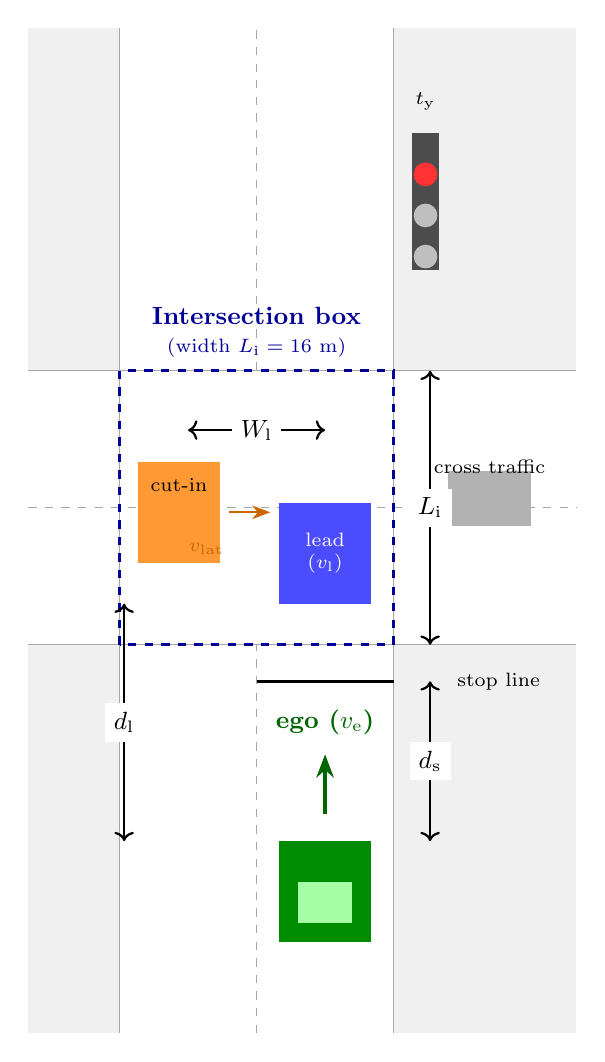
\begin{tikzpicture}[scale=0.58, every node/.style={font=\scriptsize}]
  % --- roads -------------------------------------------------------
  \fill[gray!12] (-2, -0.5) rectangle (10, 21.5);
  \fill[white]   (0, -0.5) rectangle (6, 21.5);   % ego road (northbound)
  \fill[white]   (-2, 8) rectangle (10, 14);      % crossing road
  % lane markings and road edges
  \draw[dashed, gray!70] (3, -0.5) -- (3, 8);
  \draw[dashed, gray!70] (3, 14) -- (3, 21.5);
  \draw[dashed, gray!70] (-2, 11) -- (10, 11);
  \draw[gray!70] (0, -0.5) -- (0, 21.5);
  \draw[gray!70] (6, -0.5) -- (6, 21.5);
  \draw[gray!70] (-2, 8) -- (10, 8);
  \draw[gray!70] (-2, 14) -- (10, 14);
  % --- intersection box -------------------------------------------
  \draw[very thick, blue!60!black, dashed] (0, 8) rectangle (6, 14);
  \node[blue!60!black, font=\small\bfseries] at (3, 15.2) {Intersection box};
  \node[blue!60!black, font=\scriptsize] at (3, 14.5) {(width $\Li = 16$ m)};
  % --- stop line ---------------------------------------------------
  \draw[very thick, black] (3, 7.2) -- (6, 7.2);
  \node[font=\scriptsize] at (8.3, 7.2) {stop line};
  % --- cross traffic ----------------------------------------------
  \fill[gray!60] (7.2, 10.6) rectangle (9.0, 11.8);
  \node[font=\scriptsize] at (8.1, 11.9) {cross traffic};
  % --- ego vehicle -------------------------------------------------
  \fill[green!55!black] (3.5, 1.5) rectangle (5.5, 3.7);
  \fill[green!35]       (3.9, 1.9) rectangle (5.1, 2.8);
  \draw[-{Stealth}, very thick, green!40!black] (4.5, 4.3) -- (4.5, 5.6);
  \node[green!40!black, font=\small\bfseries] at (4.5, 6.3) {ego ($\ve$)};
  % --- lead vehicle (same lane, inside the box) --------------------
  \fill[blue!70] (3.5, 8.9) rectangle (5.5, 11.1);
  \node[font=\scriptsize, white, align=center] at (4.5, 10.0) {lead\\ ($\vl$)};
  % --- cut-in vehicle (adjacent left lane) -------------------------
  \fill[orange!80] (0.4, 9.8) rectangle (2.2, 12.0);
  \node[font=\scriptsize, black, align=center] at (1.3, 11.5) {cut-in};
  \draw[-{Stealth}, thick, orange!80!black] (2.4, 10.9) -- (3.3, 10.9);
  \node[font=\scriptsize, orange!80!black] at (1.9, 10.1) {$\vlat$};
  % --- annotations --------------------------------------------------
  \draw[<->, thick] (6.8, 3.7) -- (6.8, 7.2) node[midway, fill=white, font=\small] {$\ds$};
  \draw[<->, thick] (6.8, 8) -- (6.8, 14) node[midway, fill=white, font=\small] {$\Li$};
  \draw[<->, thick] (0.1, 3.7) -- (0.1, 8.9) node[midway, fill=white, font=\small] {$\dl$};
  \draw[<->, thick] (1.5, 12.7) -- (4.5, 12.7) node[midway, fill=white, font=\small] {$\Wl$};
  % --- traffic light ------------------------------------------------
  \fill[black!70] (6.4, 16.2) rectangle (7.0, 19.2);
  \fill[red!80]   (6.7, 18.3) circle (0.26);
  \fill[gray!50]  (6.7, 17.4) circle (0.26);
  \fill[gray!50]  (6.7, 16.5) circle (0.26);
  \node[font=\scriptsize] at (6.7, 19.9) {$\tred$};
\end{tikzpicture}
\caption{Scene geometry for a northbound ego vehicle. The ego approaches a
stop line at distance $\ds$ ahead of the intersection box of width $\Li$; a
lead vehicle travelling at $\vl$ is inside the box in the ego lane; an
adjacent vehicle with an active turn signal is preparing to cut into the ego
lane from a lateral distance $\Wl$.}
\label{fig:scenario}
\end{figure}

\subsection{Stopping Distance}
\label{subsec:stopping}

The minimum distance required to bring the ego vehicle to a complete halt is
derived from the fundamental kinematic equation $v_f^2 = v_i^2 + 2 a d$.
Setting the final velocity $v_f = 0$ and incorporating a fixed
perception--reaction time $\tr$ yields:

\begin{equation}
\dreq(\ve) = \ve \cdot \tr + \frac{\ve^2}{2 \ab}.
\label{eq:stop}
\end{equation}

\textbf{Intuition.} Equation~\eqref{eq:stop} consists of two additive terms:
$\ve \tr$ is the distance travelled during the driver's reaction time, during
which no braking is applied; $\ve^2/(2\ab)$ is the pure braking distance,
derived from the work--energy principle.

\begin{theorem}[Stopping distance formula]
\label{thm:stopdist}
Under Assumptions~\ref{asm:cv}--\ref{asm:braking}, the minimum distance within
which the ego vehicle can be brought to rest, measured from the instant of
decision, is $\dreq(\ve) = \ve \tr + \ve^2/(2\ab)$.
\end{theorem}

\begin{theorem}[Stopping feasibility]
\label{thm:stopfeas}
Let $\ds$ be the distance from the ego vehicle's front bumper to the stop
line. A safe stop (Definition~\ref{def:safestop}) is physically possible if
and only if $\ds > \dreq(\ve)$.
\end{theorem}

\begin{proof}[Proof sketch]
The trajectory of the ego under maximum deceleration is
$x(t) = \ve t - \tfrac{1}{2}\ab t^2$ for $t \geq \tr$, and the stopping time
is $\tr + \ve/\ab$; the distance travelled by this time is exactly
$\dreq(\ve)$. If $\ds \leq \dreq(\ve)$, the vehicle crosses the line at
positive speed for every admissible braking profile, so no safe stop exists.
Conversely, if $\ds > \dreq(\ve)$, maximum braking halts the vehicle strictly
before the line, and the continuity of the position in the braking magnitude
(intermediate-value argument, Lemma~\ref{lem:ivt}) guarantees a profile that
stops exactly at the line. The complete argument is in
Appendix~\ref{app:proofs}.
\end{proof}

\begin{corollary}[Monotonicity]
\label{cor:mono}
$\dreq$ is strictly increasing in $\ve$, since
$\partial \dreq/\partial \ve = \tr + \ve/\ab > 0$. Higher approach speeds
strictly enlarge the stopping envelope.
\end{corollary}

\subsection{Clearance Time}
\label{subsec:clearance}

If the ego chooses to proceed, it must completely vacate the intersection
before the signal turns red. The clearance time under the constant-velocity
policy of Assumption~\ref{asm:cv} is:

\begin{equation}
\tclear(\ve, \ds) = \frac{\ds + \Li}{\ve}.
\label{eq:clear}
\end{equation}

\textbf{Intuition.} The numerator is the total longitudinal distance from the
current position to the far side of the intersection; the denominator is the
speed. Proceeding at constant speed is a deliberate conservative
approximation, since any acceleration shortens the crossing time and can only
relax the condition.

\begin{theorem}[Clearance feasibility]
\label{thm:clear}
Let $\epsilon > 0$ be the safety margin. Under the constant-velocity policy,
the ego vehicle can clear the intersection before the red phase if and only
if $\tclear(\ve, \ds) < \tred - \epsilon$.
\end{theorem}

\begin{proof}[Proof sketch]
Necessity: if $\tclear \geq \tred - \epsilon$, the constant-speed trajectory
reaches the far boundary no earlier than $\tred - \epsilon$, so it cannot
exit before the red phase. Sufficiency: if $\tclear < \tred - \epsilon$, the
far boundary is reached strictly before $\tred - \epsilon$, which itself
precedes $\tred$; the vehicle exits with margin $\epsilon$ to spare. The
margin guarantees that cross traffic has not yet entered the box.
\end{proof}

\begin{remark}
Under Assumption~\ref{asm:cv} the constant-velocity policy is the only
admissible policy, so the criterion is exact within the model. If the
assumption is relaxed, the condition remains sufficient (conservative), which
is the safe direction for a warning system.
\end{remark}

\subsection{The Dilemma Zone}
\label{subsec:dilemma}

The dilemma zone is the critical state in which neither stopping nor clearing
is possible. This is the primary scenario for which a warning must be issued.

\begin{theorem}[Dilemma zone criterion]
\label{thm:dilemma}
A \textsc{Critical} warning is necessary and sufficient if and only if:
\begin{equation}
\left( \ds \leq \dreq(\ve) \right) \;\land\;
\left( \frac{\ds + \Li}{\ve} \geq \tred - \epsilon \right).
\label{eq:dilemma}
\end{equation}
\end{theorem}

\textbf{Intuition.} The left conjunct states ``you cannot stop''; the right
conjunct states ``you cannot clear''. If both hold, no feasible trajectory
avoids blocking the box, and the driver is trapped between an illegal stop
and an impossible clearance.

\begin{proof}[Proof sketch]
\textit{Sufficiency.} Assume both conjuncts. By
Theorem~\ref{thm:stopfeas}, no braking trajectory stops before the line; by
Theorem~\ref{thm:clear}, no constant-speed trajectory clears before the red
phase. Under Assumption~\ref{asm:cv} these are the only manoeuvre classes,
so every admissible trajectory either crosses the line at positive speed or
occupies the box at $\tred - \epsilon$; in both cases the vehicle is blocked
(Definition~\ref{def:blocked}). \textit{Necessity.} If blockage is
unavoidable, a safe stop is impossible (otherwise stopping avoids blockage),
hence $\ds \leq \dreq(\ve)$; and a safe clearance is impossible (otherwise
clearing avoids blockage), hence $\tclear \geq \tred - \epsilon$.
\end{proof}

\begin{corollary}[Non-empty dilemma zone for short yellow]
\label{cor:shortyellow}
For the constants of Table~\ref{tab:notation} and $\tred = 3.5$~s, the
dilemma zone is non-empty for every speed $\ve \in (0, \infty)$, because
$\dreq(\ve) > \ve(\tred - \epsilon) - \Li$ for all $\ve$ (the quadratic
$\ve^2/8 - 1.7\ve + 16$ has negative discriminant). Consequently, at least
one warning-relevant state exists for every approach speed; see
Figure~\ref{fig:dilemma}.
\end{corollary}

\begin{figure*}[t]
\centering
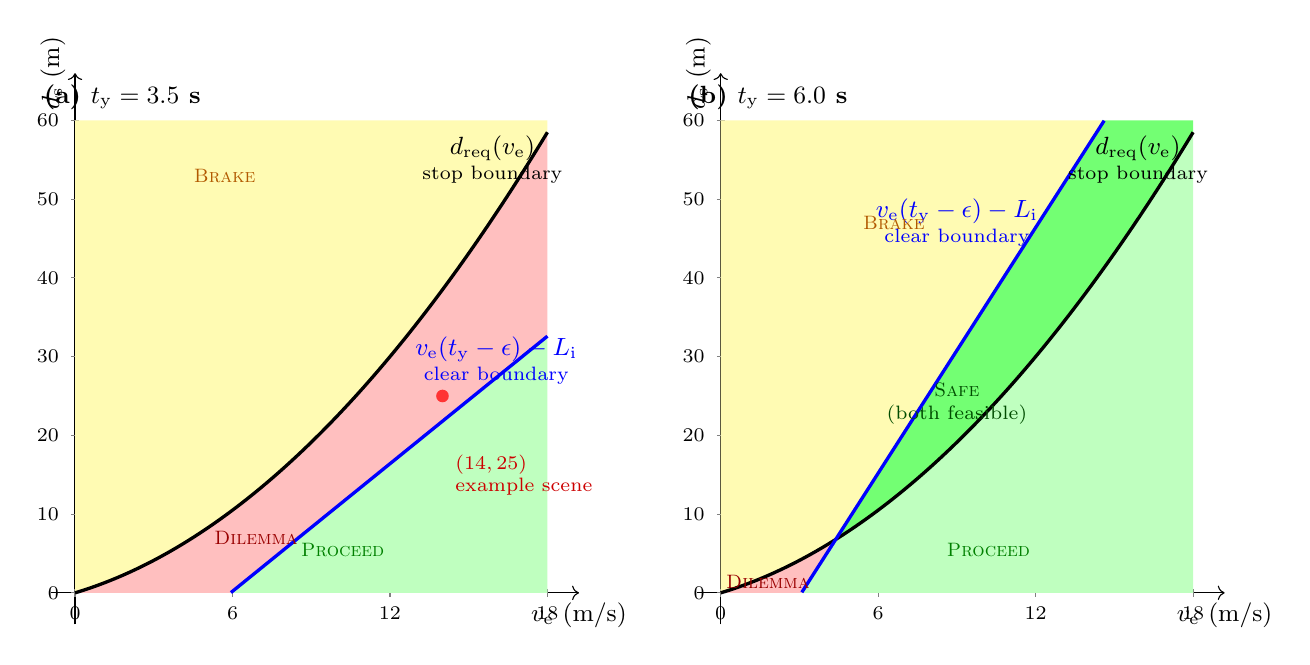
\begin{tikzpicture}[font=\small, x=1cm, y=1cm]
  % ================================================================
  % (a) t_y = 3.5 s (yellow)
  % ================================================================
  \begin{scope}[shift={(0,0)}]
    \draw[->] (-0.3,0) -- (6.4,0) node[below] {$\ve$ (m/s)};
    \draw[->] (0,-0.4) -- (0,6.6) node[left, rotate=90, anchor=south] {$\ds$ (m)};
    \foreach \v/\l in {0/0, 6/6, 12/12, 18/18} {
      \draw[gray] (\v/3, -0.05) -- (\v/3, 0.05);
      \node[below, font=\scriptsize] at (\v/3, -0.05) {$\l$};
    }
    \foreach \d/\l in {0/0, 10/10, 20/20, 30/30, 40/40, 50/50, 60/60} {
      \draw[gray] (-0.05, \d/10) -- (0.05, \d/10);
      \node[left, font=\scriptsize] at (-0.08, \d/10) {$\l$};
    }
    % region fills --------------------------------------------------
    \fill[yellow!30] (0,0) -- plot[domain=0:6, samples=80] (\x, {0.3*\x + 0.1125*\x*\x}) -- (6,6) -- (0,6) -- cycle;
    \fill[red!25] (0,0) -- (1.98,0) -- plot[domain=1.98:6, samples=40] (\x, {0.81*\x - 1.6}) -- (6,3.26) -- (6,5.85) -- plot[domain=6:0, samples=80] (\x, {0.3*\x + 0.1125*\x*\x}) -- cycle;
    \fill[green!25] (1.98,0) -- plot[domain=1.98:6, samples=40] (\x, {0.81*\x - 1.6}) -- (6,3.26) -- (6,0) -- cycle;
    % boundary curves ------------------------------------------------
    \draw[very thick, black] plot[domain=0:6, samples=80] (\x, {0.3*\x + 0.1125*\x*\x});
    \draw[very thick, blue] plot[domain=1.98:6, samples=40] (\x, {0.81*\x - 1.6});
    % labels ---------------------------------------------------------
    \node[black, align=center, font=\small] at (5.3, 5.5) {$\dreq(\ve)$\\[-2pt] {\scriptsize stop boundary}};
    \node[blue, align=center, font=\small] at (5.35, 2.95) {$\ve(\tred-\epsilon)-\Li$\\[-2pt] {\scriptsize clear boundary}};
    \node[green!50!black, align=center, font=\scriptsize] at (3.4, 0.55) {\textsc{Proceed}};
    \node[red!60!black, align=center, font=\scriptsize] at (2.3, 0.7) {\textsc{Dilemma}};
    \node[orange!70!black, align=center, font=\scriptsize] at (1.9, 5.3) {\textsc{Brake}};
    % example scene point --------------------------------------------
    \fill[red!80] (14/3, 2.5) circle (0.08);
    \node[red!80!black, font=\scriptsize, align=left] at (5.7, 1.5) {$(14, 25)$\\{\scriptsize example scene}};
    \node[font=\small\bfseries] at (0.6, 6.3) {(a) $\tred = 3.5$~s};
  \end{scope}
  % ================================================================
  % (b) t_y = 6.0 s (stale green)
  % ================================================================
  \begin{scope}[shift={(8.2,0)}]
    \draw[->] (-0.3,0) -- (6.4,0) node[below] {$\ve$ (m/s)};
    \draw[->] (0,-0.4) -- (0,6.6) node[left, rotate=90, anchor=south] {$\ds$ (m)};
    \foreach \v/\l in {0/0, 6/6, 12/12, 18/18} {
      \draw[gray] (\v/3, -0.05) -- (\v/3, 0.05);
      \node[below, font=\scriptsize] at (\v/3, -0.05) {$\l$};
    }
    \foreach \d/\l in {0/0, 10/10, 20/20, 30/30, 40/40, 50/50, 60/60} {
      \draw[gray] (-0.05, \d/10) -- (0.05, \d/10);
      \node[left, font=\scriptsize] at (-0.08, \d/10) {$\l$};
    }
    % region fills ---------------------------------------------------
    \fill[yellow!30] (0,0) -- plot[domain=0:1.46, samples=40] (\x, {0.3*\x + 0.1125*\x*\x}) -- (1.46,0.678) -- plot[domain=1.46:4.87, samples=40] (\x, {1.56*\x - 1.6}) -- (4.87,6) -- (0,6) -- cycle;
    \fill[red!25] (0,0) -- (1.03,0) -- plot[domain=1.03:1.46, samples=20] (\x, {1.56*\x - 1.6}) -- (1.46,0.678) -- plot[domain=1.46:0, samples=40] (\x, {0.3*\x + 0.1125*\x*\x}) -- cycle;
    \fill[green!25] (1.03,0) -- plot[domain=1.03:1.46, samples=20] (\x, {1.56*\x - 1.6}) -- (1.46,0.678) -- plot[domain=1.46:6, samples=80] (\x, {0.3*\x + 0.1125*\x*\x}) -- (6,5.85) -- (6,0) -- cycle;
    \fill[green!55] (1.46,0.678) -- plot[domain=1.46:4.87, samples=40] (\x, {1.56*\x - 1.6}) -- (4.87,6) -- (6,6) -- (6,5.85) -- plot[domain=6:1.46, samples=80] (\x, {0.3*\x + 0.1125*\x*\x}) -- cycle;
    % boundary curves ------------------------------------------------
    \draw[very thick, black] plot[domain=0:6, samples=80] (\x, {0.3*\x + 0.1125*\x*\x});
    \draw[very thick, blue] plot[domain=1.03:4.87, samples=40] (\x, {1.56*\x - 1.6});
    % labels ---------------------------------------------------------
    \node[black, align=center, font=\small] at (5.3, 5.5) {$\dreq(\ve)$\\[-2pt] {\scriptsize stop boundary}};
    \node[blue, align=center, font=\small] at (3.0, 4.7) {$\ve(\tred-\epsilon)-\Li$\\[-2pt] {\scriptsize clear boundary}};
    \node[green!50!black, align=center, font=\scriptsize] at (3.4, 0.55) {\textsc{Proceed}};
    \node[red!60!black, align=center, font=\scriptsize] at (0.6, 0.14) {\textsc{Dilemma}};
    \node[green!30!black, align=center, font=\scriptsize] at (3.0, 2.4) {\textsc{Safe}\\(both feasible)};
    \node[orange!70!black, align=center, font=\scriptsize] at (2.2, 4.7) {\textsc{Brake}};
    \node[font=\small\bfseries] at (0.6, 6.3) {(b) $\tred = 6.0$~s};
  \end{scope}
\end{tikzpicture}
\caption{State-space phase diagram of the dilemma zone. The black curve is
the stopping boundary $\ds = \dreq(\ve)$; the blue line is the clearance
boundary $\ds = \ve(\tred-\epsilon) - \Li$. (a) With a short yellow
($\tred = 3.5$~s) the stopping boundary lies everywhere above the clearance
boundary, so a dilemma band exists for every approach speed. (b) With a
longer green ($\tred = 6.0$~s) the clearance boundary rises above the
stopping boundary over a speed range, creating a \textsc{Safe} region in
which both stopping and clearing are feasible; the dilemma band is confined
to low speeds. The dot marks the example scene of
Section~\ref{sec:verif} ($\ve = 14$~m/s, $\ds = 25$~m), which lies inside the
dilemma band in (a).}
\label{fig:dilemma}
\end{figure*}

\subsection{Illustrative Trajectories}
\label{subsec:traj}

Figure~\ref{fig:traj} shows the three canonical outcomes for an ego vehicle
at $\ve = 12$~\si{m/s}. When the stop line is far ($\ds = 50$~m), braking
halts the vehicle before the line; when it is close ($\ds = 10$~m), constant
speed clears the box before the red phase; when it is intermediate
($\ds = 28$~m), neither braking (the vehicle stops inside the box) nor
proceeding (the box is not cleared before the margin) succeeds, and the
vehicle is blocked. This is the dilemma zone in action.

\begin{figure}[t]
\centering
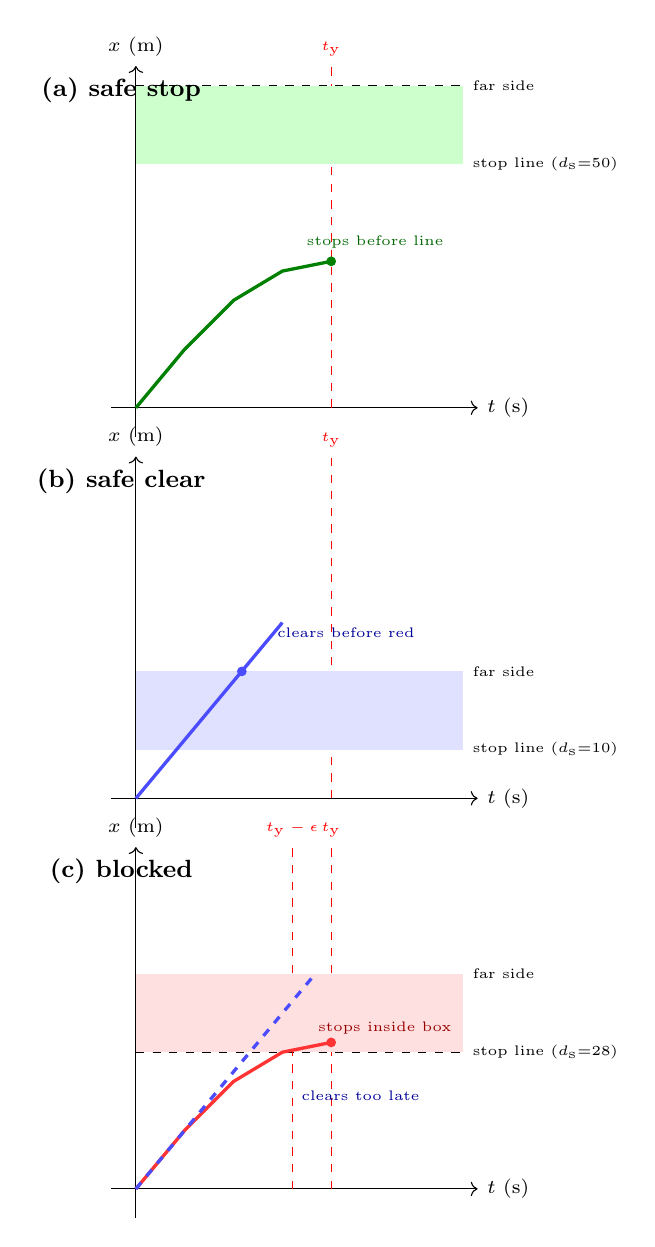
\begin{tikzpicture}[font=\scriptsize, x=0.62cm, y=0.62cm]
  % ============ (a) safe stop ============
  \begin{scope}[shift={(0,0)}]
    \draw[->] (-0.5,0) -- (7.0,0) node[right] {$t$ (s)};
    \draw[->] (0,-0.6) -- (0,7.0) node[above] {$x$ (m)};
    \draw[dashed] (0,5.0) -- (6.7,5.0);
    \node[right, font=\tiny] at (6.7,5.0) {stop line $(\ds{=}50)$};
    \draw[dashed] (0,6.6) -- (6.7,6.6);
    \node[right, font=\tiny] at (6.7,6.6) {far side};
    \draw[dashed, red] (4,0) -- (4,7.0);
    \node[above, font=\tiny, red] at (4,7.0) {$\tred$};
    \fill[green!20] (0,5.0) rectangle (6.7,6.6);
    \draw[very thick, green!50!black] (0,0) -- (1,1.2) -- (2,2.2) -- (3,2.8) -- (4,3.0);
    \fill[green!50!black] (4,3.0) circle (0.1);
    \node[green!40!black, font=\tiny] at (4.9,3.4) {stops before line};
    \node[font=\small\bfseries] at (-0.3,6.5) {(a) safe stop};
  \end{scope}
  % ============ (b) safe clear ============
  \begin{scope}[shift={(0,-8.0)}]
    \draw[->] (-0.5,0) -- (7.0,0) node[right] {$t$ (s)};
    \draw[->] (0,-0.6) -- (0,7.0) node[above] {$x$ (m)};
    \draw[dashed] (0,1.0) -- (6.7,1.0);
    \node[right, font=\tiny] at (6.7,1.0) {stop line $(\ds{=}10)$};
    \draw[dashed] (0,2.6) -- (6.7,2.6);
    \node[right, font=\tiny] at (6.7,2.6) {far side};
    \draw[dashed, red] (4,0) -- (4,7.0);
    \node[above, font=\tiny, red] at (4,7.0) {$\tred$};
    \fill[blue!12] (0,1.0) rectangle (6.7,2.6);
    \draw[very thick, blue!70] (0,0) -- (1,1.2) -- (2,2.4) -- (3,3.6);
    \fill[blue!70] (2.17,2.6) circle (0.1);
    \node[blue!60!black, font=\tiny] at (4.3,3.4) {clears before red};
    \node[font=\small\bfseries] at (-0.3,6.5) {(b) safe clear};
  \end{scope}
  % ============ (c) blocked (dilemma) ============
  \begin{scope}[shift={(0,-16.0)}]
    \draw[->] (-0.5,0) -- (7.0,0) node[right] {$t$ (s)};
    \draw[->] (0,-0.6) -- (0,7.0) node[above] {$x$ (m)};
    \draw[dashed] (0,2.8) -- (6.7,2.8);
    \node[right, font=\tiny] at (6.7,2.8) {stop line $(\ds{=}28)$};
    \draw[dashed] (0,4.4) -- (6.7,4.4);
    \node[right, font=\tiny] at (6.7,4.4) {far side};
    \draw[dashed, red] (3.2,0) -- (3.2,7.0);
    \node[above, font=\tiny, red] at (3.2,7.0) {$\tred-\epsilon$};
    \draw[dashed, red] (4,0) -- (4,7.0);
    \node[above, font=\tiny, red] at (4,7.0) {$\tred$};
    \fill[red!12] (0,2.8) rectangle (6.7,4.4);
    \draw[very thick, red!80] (0,0) -- (1,1.2) -- (2,2.2) -- (3,2.8) -- (4,3.0);
    \draw[very thick, blue!70, dashed] (0,0) -- (1,1.2) -- (2,2.4) -- (3.67,4.4);
    \fill[red!80] (4,3.0) circle (0.1);
    \node[red!60!black, font=\tiny] at (5.1,3.3) {stops inside box};
    \node[blue!60!black, font=\tiny] at (4.6,1.9) {clears too late};
    \node[font=\small\bfseries] at (-0.3,6.5) {(c) blocked};
  \end{scope}
\end{tikzpicture}
\caption{Canonical trajectories at $\ve = 12$~\si{m/s} with
$\tred = 4$~s, $\epsilon = 0.8$~s (box shaded). (a) With $\ds = 50$~m,
braking stops the vehicle before the stop line (safe stop). (b) With
$\ds = 10$~m, constant speed clears the far side at $t = 2.17$~s, before
$\tred - \epsilon = 3.2$~s (safe clear). (c) With $\ds = 28$~m, braking
stops the vehicle at $x = 30$~m, inside the box, while the constant-speed
policy clears only at $t = 3.67$~s, after the margin. Neither policy avoids
blockage: the state is in the dilemma zone.}
\label{fig:traj}
\end{figure}

\subsection{Lead Vehicle Constraint}
\label{subsec:lead}

A slower leading vehicle imposes an upper bound on the ego's effective speed:
the ego cannot pass the leader, so the time to clear the intersection is
governed by the leader's motion.

\begin{definition}[Effective clearance time]
\label{def:effclear}
Given a lead vehicle at distance $\dl$ with speed $\vl$, the effective
clearance time is
\begin{equation}
\teff = \frac{\dl + \Li}{\vl + \delta},
\label{eq:eff_clear}
\end{equation}
where $\delta$ is a small positive constant that prevents division by zero.
\end{definition}

\begin{theorem}[Following blockage]
\label{thm:follow}
If $\teff \geq \tred - \epsilon$ and $\dl < \dreq(\ve)$, the ego vehicle will
become trapped behind the leader and block the intersection.
\end{theorem}

\textbf{Intuition.} Even if the ego has sufficient speed to clear the
intersection alone, the leader's slow speed acts as a moving blockage. The
ego must follow at the leader's speed; if the leader has not cleared the box
by the time the light turns red, the ego is stuck directly behind it, still
inside the box.

\begin{proof}[Proof sketch]
The ego's longitudinal position is constrained by the collision-avoidance
requirement $x_{\mathrm{ego}}(t) < x_{\mathrm{lead}}(t)$. The earliest time
at which the ego can reach the far side of the box is when the leader has
cleared it, which requires $t = \teff$. If $\teff \geq \tred - \epsilon$, the
leader still occupies the box at the red phase and so does the ego. The
second condition $\dl < \dreq(\ve)$ rules out aborting: the ego cannot stop
behind the leader, because the gap is smaller than its stopping distance.
Hence blockage is unavoidable.
\end{proof}

\begin{remark}[Lead-vehicle operational boundary]
\label{rem:leadbound}
The guarantee of Theorem~\ref{thm:follow} is conditional on the leader's
motion: it holds provided the leader does not decelerate beyond a worst-case
bound. Under Assumption~\ref{asm:cv} this bound is effectively zero, since the
leader maintains constant velocity. For deployment we recommend a conservative
bound of $a_{\mathrm{lead}} = 0.4\,g \approx 3.9$~\si{m/s^2}, so that the
effective clearance time becomes
$\teff = (\dl + \Li)\,/\,\max\bigl(0.1,\; \vl - a_{\mathrm{lead}}\,(\tred - \epsilon)\bigr)$.
Within this defined operational envelope the warning remains sound; outside it,
the system degrades gracefully rather than claiming certainty.
\end{remark}

\subsection{Lane-Changing Constraint}
\label{subsec:cutin}

Adjacent vehicles that signal and move laterally into the ego's lane reduce
the available stopping distance and invalidate the previously computed
geometry.

\begin{definition}[Time to intrusion]
\label{def:intrusion}
Let $\vlat$ be the lateral speed of an adjacent vehicle. The time for it to
cross into the ego's lane is
\begin{equation}
\tint = \frac{\Wl}{|\vlat|},
\label{eq:intrude}
\end{equation}
where $\Wl = 3.5$~m is the standard lane width.
\end{definition}

\begin{theorem}[Cut-in warning]
\label{thm:cutin}
Let $\da$ be the distance to an adjacent vehicle with an active turn signal.
If $\tint < \tred$ and $\da < \dreq(\ve)$, then the ego must issue a warning.
\end{theorem}

\textbf{Intuition.} The adjacent vehicle will intrude into the ego's path
before the light changes, effectively creating a new, closer lead vehicle.
The ego's previously computed stopping distance is then invalid; the new
stopping requirement cannot be met, making a collision or blockage imminent.

\begin{proof}[Proof sketch]
If $\tint < \tred$, the lane change occurs before the signal transition. At
the moment of intrusion the longitudinal gap becomes $\da$, and since
$\da < \dreq(\ve)$ the ego cannot stop before reaching the cutting vehicle.
If the ego brakes, it either stops beyond the stop line or collides; if it
proceeds, it must clear the box while the intruder occupies the lane. In
either case the kinematic constraints are violated, so a warning is required.
\end{proof}

\subsection{Signal-State and Advisory Rules}
\label{subsec:signal}

Two operational rules complete the criterion set. First, an observed red
signal makes blockage imminent by definition and must produce a
\textsc{Critical} warning. A yellow signal with $\tred < 2.5$~s leaves
insufficient time for a safe stop in most traffic and produces a
\textsc{Caution}. Second, a stale-green heuristic issues a \textsc{Caution}
when the green phase has been active long enough that the driver should
prepare for a possible transition while still at a distance
$\ds > \dreq(\ve)$ (i.e., while stopping remains feasible). These rules are
stated directly in the implementation (Section~\ref{sec:arch}) rather than as
additional theorems, since they encode operational policy rather than
kinematic law.

\section{System Architecture}
\label{sec:arch}

The implementation is structured into four modules, each adhering to the
Single Responsibility Principle (SRP). The decision engine is a functional
pipeline that composes five independent checkers in descending severity order
(Figure~\ref{fig:arch}).

\begin{figure*}[t]
\centering
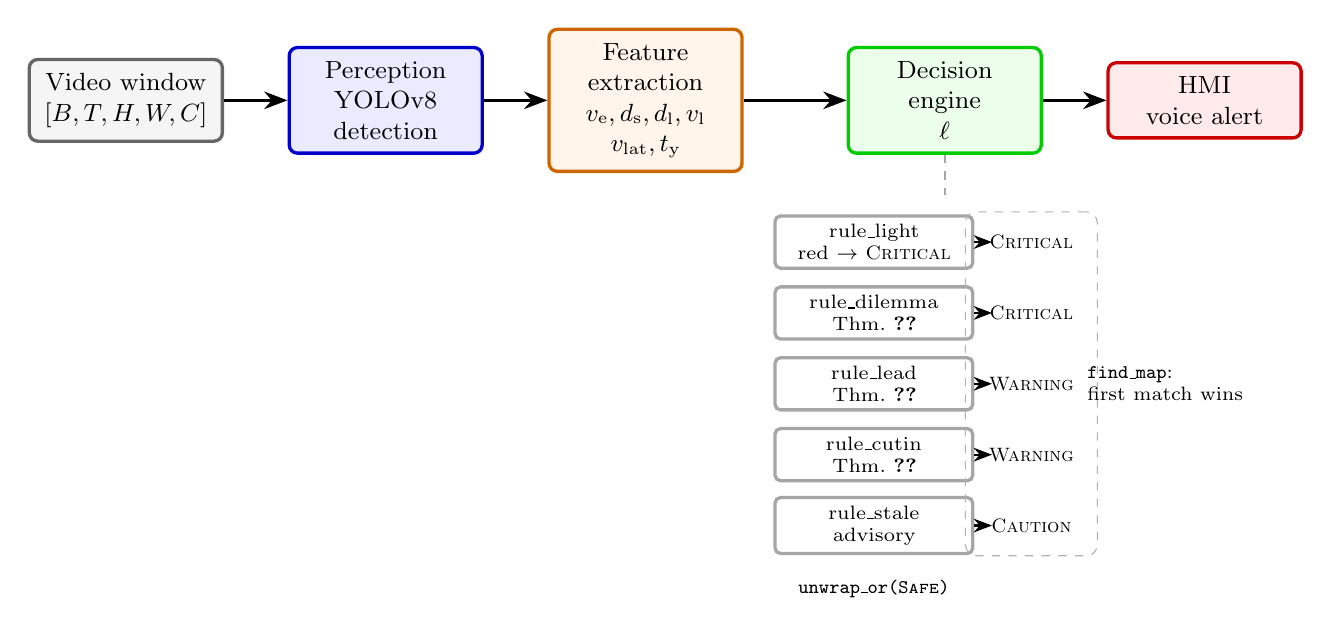
\begin{tikzpicture}[
  font=\small,
  >=Stealth,
  box/.style={draw=#1!80!black, very thick, rounded corners=3pt,
              fill=#1!8, align=center, inner sep=5pt, text width=2.1cm},
  pipe/.style={draw=gray!70, very thick, rounded corners=2pt, align=center,
               inner sep=3pt, text width=2.3cm, font=\scriptsize},
  chip/.style={font=\scriptsize, align=left},
]
  % --- pipeline stages --------------------------------------------
  \node[box=gray] (cam) at (0,0) {Video window\\$[B,T,H,W,C]$};
  \node[box=blue] (perc) at (3.3,0) {Perception\\YOLOv8\\detection};
  \node[box=orange] (feat) at (6.6,0) {Feature\\extraction\\$\ve,\ds,\dl,\vl$\\$\vlat,\tred$};
  \node[box=green] (dec) at (10.4,0) {Decision\\engine\\$\ell$};
  \node[box=red] (out) at (13.7,0) {HMI\\voice alert};

  \draw[->, very thick] (cam) -- (perc);
  \draw[->, very thick] (perc) -- (feat);
  \draw[->, very thick] (feat) -- (dec);
  \draw[->, very thick] (dec) -- (out);

  % --- expanded decision engine (below) ---------------------------
  \draw[gray!70, dashed, thick] (dec.south) -- (10.4, -1.2);

  \node[pipe] (r1) at (9.5, -1.8) {rule\_light\\red $\to$ \textsc{Critical}};
  \node[pipe] (r2) at (9.5, -2.7) {rule\_dilemma\\Thm.~\ref{thm:dilemma}};
  \node[pipe] (r3) at (9.5, -3.6) {rule\_lead\\Thm.~\ref{thm:follow}};
  \node[pipe] (r4) at (9.5, -4.5) {rule\_cutin\\Thm.~\ref{thm:cutin}};
  \node[pipe] (r5) at (9.5, -5.4) {rule\_stale\\advisory};

  \node[chip] (c1) at (11.5, -1.8) {\textsc{Critical}};
  \node[chip] (c2) at (11.5, -2.7) {\textsc{Critical}};
  \node[chip] (c3) at (11.5, -3.6) {\textsc{Warning}};
  \node[chip] (c4) at (11.5, -4.5) {\textsc{Warning}};
  \node[chip] (c5) at (11.5, -5.4) {\textsc{Caution}};

  \draw[->, thick] (r1.east) -- (11.0, -1.8);
  \draw[->, thick] (r2.east) -- (11.0, -2.7);
  \draw[->, thick] (r3.east) -- (11.0, -3.6);
  \draw[->, thick] (r4.east) -- (11.0, -4.5);
  \draw[->, thick] (r5.east) -- (11.0, -5.4);

  \node[draw=gray!60, dashed, rounded corners=4pt, fit=(c1)(c2)(c3)(c4)(c5),
        inner sep=5pt] {};
  \node[font=\scriptsize, align=left] at (13.2, -3.6) {\texttt{find\_map}:\\first match wins};
  \node[font=\scriptsize, align=center] at (9.5, -6.2) {\texttt{unwrap\_or(\textsc{Safe})}};
\end{tikzpicture}
\caption{System architecture. Raw frames are processed by the perception
layer into physical quantities; the decision engine evaluates five
single-responsibility rules in descending severity order and returns the
first match (or \textsc{Safe} if none fires).}
\label{fig:arch}
\end{figure*}

\subsection{Module: \texttt{models.rs}}
\label{sub:models}
This module defines immutable data structures and exhaustive enums. All
types are copy-able and side-effect free.

\begin{lstlisting}[language=Rust, caption=src/models.rs]
//! Core data types representing the state of the traffic scene.
//! All types are immutable; transformations produce new instances.

/// The current colour of the traffic light.
#[derive(Debug, Clone, Copy, PartialEq, Eq)]
pub enum LightState {
    Red,
    Yellow,
    Green,
    Unknown, // Sensor failure.
}

/// Lane position relative to the ego vehicle.
#[derive(Debug, Clone, Copy, PartialEq, Eq)]
pub enum LanePosition {
    Same,
    Left,
    Right,
    Unknown,
}

/// The severity of the warning issued to the driver.
#[derive(Debug, Clone, Copy, PartialEq, Eq, PartialOrd, Ord)]
pub enum WarningLevel {
    Safe,
    Caution,
    Warning,
    Critical,
}

/// A tracked object from the perception pipeline.
#[derive(Debug, Clone)]
pub struct Detection {
    pub bbox: (f32, f32, f32, f32),
    pub class_id: u8,
    pub speed: f32,
    pub lateral_speed: f32,
    pub distance_to_ego: f32,
    pub lane: LanePosition,
    pub turn_signal_active: bool,
}

impl Detection {
    /// Returns `true` if the detection belongs to a vehicle class.
    #[must_use]
    pub fn is_vehicle(&self) -> bool {
        matches!(self.class_id, 2 | 3 | 5 | 7)
    }
}

/// State of the ego vehicle.
#[derive(Debug, Clone, Copy)]
pub struct EgoState {
    pub speed: f32,
    pub distance_to_stop_line: f32,
}

/// Derived state of the closest lead vehicle.
#[derive(Debug, Clone, Copy)]
pub struct LeadVehicle {
    pub distance: f32,
    pub speed: f32,
    pub is_in_intersection: bool,
}
\end{lstlisting}

\subsection{Module: \texttt{algebra.rs}}
\label{sub:algebra}
This module contains only pure functions implementing the kinematic
equations of Section~\ref{sec:kinematics}. No decision logic is present.

\begin{lstlisting}[language=Rust, caption=src/algebra.rs]
//! Pure algebraic functions for kinematic calculations.
//! These are stateless, deterministic, and side-effect-free.

/// Physical constants derived from automotive safety standards.
pub mod constants {
    /// Maximum comfortable deceleration (m/s^2).
    pub const MAX_DECEL: f32 = 4.0;
    /// Perception-reaction time (seconds).
    pub const REACTION_TIME: f32 = 1.0;
    /// Standard intersection width for two lanes (meters).
    pub const INTERSECTION_LENGTH: f32 = 16.0;
    /// Safety margin to guarantee red phase clearance (seconds).
    pub const SAFETY_MARGIN: f32 = 0.8;
    /// Small epsilon to prevent division by zero.
    pub const EPSILON: f32 = 0.1;
    /// Standard lane width for cut-in calculations (meters).
    pub const LANE_WIDTH: f32 = 3.5;
}

/// Computes the minimum stopping distance (Eq. 1).
///
/// # Derivation
/// From `v_f^2 = v_i^2 + 2*a*d`, with `v_f = 0` and `a = -MAX_DECEL`,
/// we obtain `d_brake = v^2 / (2 * MAX_DECEL)`. Adding the reaction
/// distance `v * REACTION_TIME` yields the total.
///
/// # Arguments
/// * `ego_speed` - Current longitudinal velocity (m/s).
///
/// # Returns
/// The distance (m) required to achieve a full stop.
#[must_use]
pub fn stopping_distance(ego_speed: f32) -> f32 {
    let reaction_dist = ego_speed * constants::REACTION_TIME;
    let braking_dist = (ego_speed * ego_speed) / (2.0 * constants::MAX_DECEL);
    reaction_dist + braking_dist
}

/// Computes the time to clear the intersection (Eq. 2).
///
/// # Arguments
/// * `distance_to_line` - Distance from front bumper to the stop line (m).
/// * `speed` - Current longitudinal velocity (m/s).
///
/// # Returns
/// The time (s) required to reach the far side of the intersection.
#[must_use]
pub fn clearance_time(distance_to_line: f32, speed: f32) -> f32 {
    let denominator = speed + constants::EPSILON;
    (distance_to_line + constants::INTERSECTION_LENGTH) / denominator
}

/// Computes the time for an adjacent vehicle to intrude into the ego lane
/// (Eq. 4).
///
/// # Arguments
/// * `lateral_speed` - The lateral velocity of the adjacent vehicle (m/s).
///
/// # Returns
/// The time (s) until the lane boundary is crossed.
#[must_use]
pub fn intrusion_time(lateral_speed: f32) -> f32 {
    constants::LANE_WIDTH / (lateral_speed.abs() + constants::EPSILON)
}
\end{lstlisting}

\subsection{Module: \texttt{rules.rs}}
\label{sub:rules}
This module contains five single-responsibility functions. Each function
takes the relevant state and returns \texttt{Option<WarningLevel>}; they are
completely independent and deterministic.

\begin{lstlisting}[language=Rust, caption=src/rules.rs]
//! Decision rules. Each function implements one criterion of
//! Section 4. All functions are pure and return `Option` to
//! facilitate composition.

use crate::algebra::*;
use crate::models::*;

/// Rule 1 (Section 4.6): Light state rule.
/// Red implies Critical; short yellow implies Caution.
#[must_use]
pub fn rule_light(light: LightState, time_to_red: f32) -> Option<WarningLevel> {
    match light {
        LightState::Red => Some(WarningLevel::Critical),
        LightState::Yellow if time_to_red < 2.5 => Some(WarningLevel::Caution),
        _ => None,
    }
}

/// Rule 2 (Theorem 4): Dilemma zone rule.
/// The core stopping-clearance conjunction.
#[must_use]
pub fn rule_dilemma(ego: &EgoState, time_to_red: f32) -> Option<WarningLevel> {
    let d_req = stopping_distance(ego.speed);
    let t_c = clearance_time(ego.distance_to_stop_line, ego.speed);

    let cannot_stop = ego.distance_to_stop_line <= d_req;
    let cannot_clear = t_c >= (time_to_red - constants::SAFETY_MARGIN);

    match (cannot_stop, cannot_clear) {
        (true, true) => Some(WarningLevel::Critical),
        _ => None,
    }
}

/// Rule 3 (Theorem 5): Lead vehicle rule.
/// Checks if the leader is stopped in the box or if following it
/// causes a clearance failure.
#[must_use]
pub fn rule_lead(ego_speed: f32, lead: &LeadVehicle, time_to_red: f32) -> Option<WarningLevel> {
    let d_req = stopping_distance(ego_speed);

    // Sub-rule 3a: leader is stopped and already inside the intersection.
    if lead.speed < 1.0 && lead.distance < d_req && lead.is_in_intersection {
        return Some(WarningLevel::Critical);
    }

    // Sub-rule 3b: following the leader causes a clearance failure.
    let t_eff = clearance_time(lead.distance, lead.speed);
    if t_eff >= (time_to_red - constants::SAFETY_MARGIN) && lead.distance < d_req {
        return Some(WarningLevel::Warning);
    }

    None
}

/// Rule 4 (Theorem 6): Cut-in rule.
/// Detects adjacent vehicles with turn signals that will intrude
/// before the light changes.
#[must_use]
pub fn rule_cutin(detections: &[Detection], ego_speed: f32, time_to_red: f32) -> Option<WarningLevel> {
    let d_req = stopping_distance(ego_speed);

    detections
        .iter()
        .filter(|d| d.is_vehicle() && d.turn_signal_active && d.lane != LanePosition::Same)
        .find(|d| {
            let t_intrude = intrusion_time(d.lateral_speed);
            t_intrude < time_to_red && d.distance_to_ego < d_req
        })
        .map(|_| WarningLevel::Warning)
}

/// Rule 5 (Section 4.6): Stale-green heuristic.
/// Advises Caution when the green has been active long enough.
#[must_use]
pub fn rule_stale(light: LightState, ego: &EgoState) -> Option<WarningLevel> {
    match light {
        LightState::Green if ego.distance_to_stop_line > stopping_distance(ego.speed) => {
            Some(WarningLevel::Caution)
        }
        _ => None,
    }
}
\end{lstlisting}

\subsection{Module: \texttt{decision.rs}}
\label{sub:decision}
The orchestrator composes the rules using a functional pipeline
(Figure~\ref{fig:arch}). The pipeline is deliberately ordered by descending
severity so that the first matching rule is always the most urgent one.

\begin{lstlisting}[language=Rust, caption=src/decision.rs]
//! Decision engine pipeline. Composes five rules.
//! Adding a new rule requires inserting it into the vector.

use crate::algebra::constants;
use crate::models::*;
use crate::rules::*;

/// Evaluates the entire traffic scene and returns the highest-priority
/// warning.
///
/// # Pipeline design
/// Rules are ordered by descending severity: red light and the dilemma
/// zone (Critical) precede the lead and cut-in rules (Warning), which
/// precede the stale-green heuristic (Caution). `find_map` returns the
/// first rule that fires; `unwrap_or(Safe)` covers the no-warning case.
#[must_use]
pub fn evaluate_safety(
    ego: &EgoState,
    detections: &[Detection],
    light: LightState,
    time_to_red: f32,
) -> WarningLevel {
    // Extract the lead vehicle from detections.
    let lead_opt = detections
        .iter()
        .find(|d| d.is_vehicle() && d.lane == LanePosition::Same)
        .map(|d| LeadVehicle {
            distance: d.distance_to_ego,
            speed: d.speed,
            is_in_intersection: d.distance_to_ego < constants::INTERSECTION_LENGTH,
        });

    // Build the severity-ordered pipeline.
    let rules: Vec<Box<dyn Fn() -> Option<WarningLevel>>> = vec![
        Box::new(|| rule_light(light, time_to_red)),
        Box::new(|| rule_dilemma(ego, time_to_red)),
        Box::new(|| lead_opt.and_then(|l| rule_lead(ego.speed, &l, time_to_red))),
        Box::new(|| rule_cutin(detections, ego.speed, time_to_red)),
        Box::new(|| rule_stale(light, ego)),
    ];

    // Execute the pipeline; the first matching rule determines the level.
    rules
        .into_iter()
        .find_map(|rule| rule())
        .unwrap_or(WarningLevel::Safe)
}
\end{lstlisting}

\subsection{Entry Point (\texttt{main.rs}) and Manifest}

\begin{lstlisting}[language=Rust, caption=src/main.rs]
mod algebra;
mod models;
mod rules;
mod decision;

use decision::evaluate_safety;
use models::*;

fn main() {
    // Simulated sensor inputs (dilemma-zone scene).
    let ego = EgoState { speed: 14.0, distance_to_stop_line: 25.0 };
    let detections = vec![
        Detection { bbox: (0.0,0.0,0.0,0.0), class_id: 2, speed: 5.0,
            lateral_speed: 0.0, distance_to_ego: 20.0,
            lane: LanePosition::Same, turn_signal_active: false },
        Detection { bbox: (0.0,0.0,0.0,0.0), class_id: 2, speed: 18.0,
            lateral_speed: 1.2, distance_to_ego: 15.0,
            lane: LanePosition::Left, turn_signal_active: true },
    ];

    let result = evaluate_safety(&ego, &detections, LightState::Yellow, 3.5);
    println!("Decision: {:?}", result); // Outputs: Critical
}
\end{lstlisting}

\begin{lstlisting}[caption=Cargo.toml]
[package]
name = "intersection-rs"
version = "0.1.0"
edition = "2021"

[dependencies]
# No external crates required for the core decision engine.
# For perception, integrate with opencv-rs or tch-rs externally.
\end{lstlisting}

\section{Verification}
\label{sec:verif}

Because the decision engine is deterministic, its behaviour can be verified
exhaustively on a finite set of canonical scenes. Table~\ref{tab:scenarios}
enumerates representative test vectors together with the rule that fires and
the expected warning level. Each row is an executable test case: the
functions of Section~\ref{sec:arch} return exactly the stated level.

\begin{table}[t]
\caption{Canonical verification scenarios (constants of
Table~\ref{tab:notation}).}
\label{tab:scenarios}
\centering
\footnotesize
\begin{tabular}{@{}cllc@{}}
\toprule
\# & Scene summary & Firing rule & Expected level \\
\midrule
1 & Red light, any state & rule\_light & \textsc{Critical} \\
2 & Yellow, $\tred=1.5$~s & rule\_light & \textsc{Caution} \\
3 & Dilemma zone, $\ve{=}14$, $\ds{=}25$ & rule\_dilemma & \textsc{Critical} \\
4 & Lead stopped inside box & rule\_lead (3a) & \textsc{Critical} \\
5 & Slow lead, $\vl{=}5$, $\dl{=}20$ & rule\_lead (3b) & \textsc{Warning} \\
6 & Cut-in vehicle, $\vlat{=}1.2$, $\da{=}15$ & rule\_cutin & \textsc{Warning} \\
7 & Stale green, far from line & rule\_stale & \textsc{Caution} \\
8 & Green, comfortable stop margin & none & \textsc{Safe} \\
\bottomrule
\end{tabular}
\end{table}

\paragraph{Complexity.} The pipeline evaluates each rule at most once, and
only \texttt{rule\_cutin} iterates over the detection list, so the decision
engine is $O(n)$ per frame, where $n$ is the number of detections. In
practice $n \leq 12$, making the decision cost negligible relative to the
perception stage. The overall per-frame complexity is dominated by the
object detector.

\section{Discussion}
\label{sec:discussion}

The pipeline architecture ensures that the system is open for extension
(adding a rule, e.g., for pedestrian detection) but closed for modification.
Pure functions and immutable data eliminate entire classes of runtime errors
related to mutable state; exhaustive pattern matching on \texttt{LightState}
and \texttt{LanePosition} forces explicit handling of every sensor failure
mode, and the severity-ordered composition makes the priority semantics
visible in code.

\paragraph{Safety engineering.} Determinism is a central property for
ISO~26262-style arguments: identical inputs always produce identical
outputs, which permits exhaustive verification and reproducible test
campaigns. All constants in Table~\ref{tab:notation} are either
standardised or configurable, and the proofs in
Appendix~\ref{app:proofs} establish that the rules fire exactly when the
corresponding kinematic condition holds. There is no learned ``hidden
logic'' to audit. Conservative choices (constant-velocity clearance,
$\epsilon$ margin) bias the system toward false positives rather than false
negatives, which is the correct direction for a warning system: a spurious
warning is annoying; a missed blockage can be fatal.

\begin{figure*}[t]
\centering
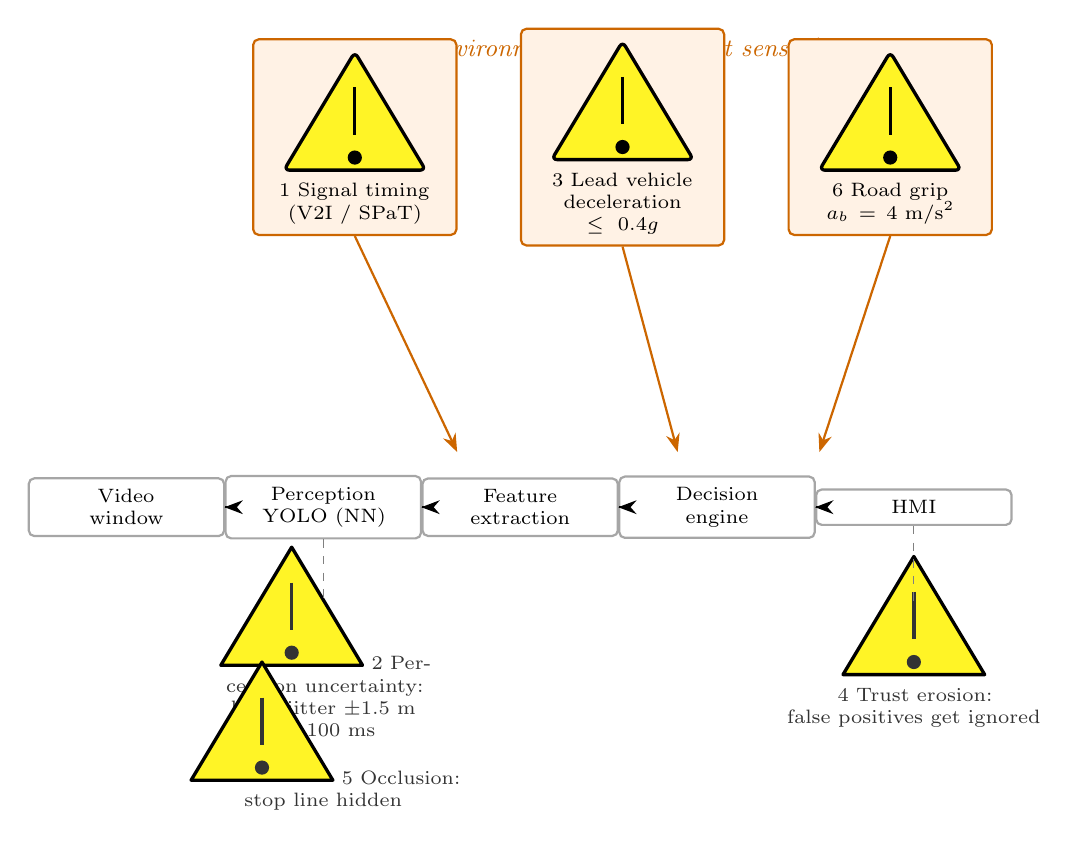
\begin{tikzpicture}[
  font=\scriptsize,
  >=Stealth,
  envbox/.style={draw=orange!80!black, thick, rounded corners=2pt, align=center,
                 inner sep=4pt, text width=2.3cm, fill=orange!10},
  pbox/.style={draw=gray!70, thick, rounded corners=2pt, align=center,
               inner sep=4pt, text width=2.2cm},
  wnote/.style={align=center, text width=3.4cm, font=\scriptsize, text=black!80},
]
  % environment row
  \node[font=\small\itshape, text=orange!80!black] at (6.3, 5.8) {Environment (assumed, not sensed)};
  \node[envbox] (e1) at (2.9, 4.7) {\warnicon\ 1 Signal timing\\ (V2I / SPaT)};
  \node[envbox] (e2) at (6.3, 4.7) {\warnicon\ 3 Lead vehicle\\ deceleration $\leq 0.4g$};
  \node[envbox] (e3) at (9.7, 4.7) {\warnicon\ 6 Road grip\\ $a_b = 4$~m/s$^2$};
  % pipeline row
  \node[pbox] (p1) at (0, 0) {Video\\window};
  \node[pbox] (p2) at (2.5, 0) {Perception\\YOLO (NN)};
  \node[pbox] (p3) at (5.0, 0) {Feature\\extraction};
  \node[pbox] (p4) at (7.5, 0) {Decision\\engine};
  \node[pbox] (p5) at (10.0, 0) {HMI};
  \draw[->, thick] (p1) -- (p2);
  \draw[->, thick] (p2) -- (p3);
  \draw[->, thick] (p3) -- (p4);
  \draw[->, thick] (p4) -- (p5);
  % environment feeds the decision chain
  \draw[->, thick, orange!80!black] (e1.south) -- (4.2, 0.7);
  \draw[->, thick, orange!80!black] (e2.south) -- (7.0, 0.7);
  \draw[->, thick, orange!80!black] (e3.south) -- (8.8, 0.7);
  % warnings below the pipeline
  \node[wnote] (w2) at (2.5, -1.7) {\warnicon\ 2 Perception uncertainty:\\ bbox jitter $\pm 1.5$~m $\approx 100$~ms};
  \node[wnote] (w5) at (2.5, -2.9) {\warnicon\ 5 Occlusion:\\ stop line hidden};
  \node[wnote] (w4) at (10.0, -1.7) {\warnicon\ 4 Trust erosion:\\ false positives get ignored};
  \draw[dashed, gray] (p2.south) -- (2.5, -1.25);
  \draw[dashed, gray] (p5.south) -- (10.0, -1.25);
\end{tikzpicture}
\caption{Known vulnerabilities mapped onto the system pipeline. The three
environmental quantities (signal timing, lead-vehicle motion, road grip) are
assumed rather than sensed and enter the formal guarantees as explicit bounds;
the perception-stage vulnerabilities affect the accuracy of the inputs; the
HMI-stage vulnerability affects whether warnings are obeyed. Numbered icons
match the discussion in Section~\ref{sec:discussion}.}
\label{fig:vuln}
\end{figure*}

\paragraph{\warnicon~Known vulnerabilities and operational boundaries.}
Peer review of an earlier draft surfaced six concerns that we state explicitly
rather than hide.
Figure~\ref{fig:vuln} maps each vulnerability onto the pipeline stage where it
enters.
\warnicon~\textbf{(1) Signal timing.} Without V2I or a SPaT (signal phase and timing)
feed, a vision-only system cannot know when a stale green turns yellow;
Remark~\ref{rem:worstcase} applies, and the ``stale'' aspect of the warning
reduces to pure geometry.
\warnicon~\textbf{(2) Perception uncertainty.} Neural network outputs are point
estimates, and a confidence score is not a formal bound. A bounding-box
jitter of $\pm 1.5$~m at $14$~m/s shifts the arrival-time estimate by roughly
$100$~ms, which can flip a safe decision into a blocked one. The formal
results therefore hold for the given inputs, not for the unobserved ground
truth.
\warnicon~\textbf{(3) Lead-vehicle motion.} Theorem~\ref{thm:follow} is conditional on
a bounded leader deceleration (Remark~\ref{rem:leadbound}); the operational
envelope is defined by that bound.
\warnicon~\textbf{(4) HMI trust.} Frequent false positives erode driver trust and can
cause the system to be ignored, turning the next missed warning into a fatal
outcome. The threshold policy is therefore recall-first, minimizing false
negatives, and future work targets a dynamic threshold adapted to the
driver's reaction time, with warning intensity modulated by confidence.
\warnicon~\textbf{(5) Occlusion.} A large vehicle can hide the stop line or the lead
vehicle entirely; such detection gaps lie outside the formal scope.
\warnicon~\textbf{(6) Road friction.} Assumption~\ref{asm:braking} fixes grip at
$4.0$~\si{m/s^2}; wet or icy surfaces reduce it, and the stopping envelope
must be re-tuned for the local condition.

\paragraph{Scope of the formal results.} The proofs establish properties of
the decision logic given exact inputs. They do not bound perception error,
signal-timing uncertainty, or actuator performance. Each theorem is a
conditional statement: if the inputs satisfy the assumptions, the output is
correct. Guaranteeing the inputs themselves (object detection, tracking,
signal timing) is a perception problem, and the deterministic engine is
deliberately agnostic to how the inputs are obtained. Moving the physical
bounds into the type system (e.g., constructors that reject impossible
speeds or distances) is planned future work and would push a further part of
this verification into the compiler.

\paragraph{Pedagogical use case.} Because the engine is white box, the HMI
can display the violated constraint directly, for example ``you are braking
at $0.3\,g$, you need $0.5\,g$ to stop before the line''. This turns a
warning into an explanation, which is valuable for student drivers and
differentiates the system from OEM ADAS that treat the driver as a passive
monitor.

\paragraph{Limitations.} The framework inherits the limitations of its
assumptions. Assumption~\ref{asm:cv} ignores acceleration and deceleration
by surrounding vehicles; Assumption~\ref{asm:signal} requires signal-timing
observability; and Assumption~\ref{asm:braking} assumes nominal friction.
Sensor noise in the perception layer propagates into the physical estimates,
and although the decision logic is deterministic, the measurements feeding
it are not. These limitations motivate several lines of future work:
(i)~probabilistic propagation of measurement uncertainty, via Kalman-filter
covariances or interval arithmetic, through the kinematic equations to
produce calibrated confidence levels for each warning; (ii)~dynamic warning
thresholds adapted to the driver's reaction time; (iii)~extension of the
rule set to vulnerable road users and multi-lane crossing scenes; and
(iv)~type-level enforcement of physical bounds. The deterministic core is
the correct foundation for all of these, since probabilistic extensions can
be layered on top without changing the underlying kinematics.

\section{Conclusion}
\label{sec:conclusion}
A deterministic, mathematically proven system for intersection blockage
prediction has been presented. The method requires no labelled data and
provides interpretable warnings based on violated kinematic constraints,
formalised in five theorems with complete proofs
(Appendix~\ref{app:proofs}), valid within an explicitly defined operational
envelope (Section~\ref{sec:discussion}). The Rust implementation is modular,
SOLID-compliant, dependency-free, and severity-ordered, with $O(n)$ per-frame
cost and exhaustive handling of sensor states. Source listings, this paper,
and the proofs appendix are available online.

\section*{Acknowledgment}
The author thanks the CivicSense community for field data and feedback.
Source code, this paper (PDF and \LaTeX{}), and the HTML proofs appendix are
available at
\url{https://github.com/arpanpathak/driving-civicsense-vision-model/tree/main/research_paper}
and rendered at
\url{https://arpanpathak.github.io/driving-civicsense-vision-model/}.

% ==================================================================
% Appendix: complete proofs
% ==================================================================
\appendices
\section{Complete Mathematical Proofs}
\label{app:proofs}

This appendix develops the formal results of Section~\ref{sec:kinematics}
self-contained. We first prove supporting lemmas, then restate and prove each
theorem in full. Throughout, time is measured in seconds, distances in
metres, speeds in \si{m/s}, and accelerations in \si{m/s^2}. We assume the
kinematic model of Assumptions~\ref{asm:cv}--\ref{asm:braking}: longitudinal
motion is governed by $\ddot{x} = a(t)$ with $|a(t)| \leq \ab$ and an
actuation delay $\tr$ during which $a(t) = 0$.

\paragraph{Scope of the proofs.}
Every result below is a conditional statement: given exact inputs that
satisfy the stated assumptions, the conclusion follows. The proofs do not
bound perception error, signal-timing uncertainty, or actuator performance,
and they do not assert that the measured inputs equal the ground truth. The
formal guarantee therefore covers the decision logic itself, not the
perception chain that feeds it.

\subsection{Supporting Lemmas}

\begin{lemma}[Braking distance]
\label{lem:brakedist}
Under constant deceleration $\ab$ from initial speed $\ve$, the distance
travelled until rest is $\ve^2 / (2\ab)$.
\end{lemma}

\begin{proof}
The equation of motion during braking is $\ddot{x} = -\ab$, with initial
conditions $x(0)=0$, $\dot{x}(0)=\ve$. Integrating twice:
$\dot{x}(t) = \ve - \ab t$ and
$x(t) = \ve t - \tfrac{1}{2}\ab t^2$. The vehicle is at rest when
$\dot{x}(t_s) = 0$, i.e.\ $t_s = \ve/\ab$. Substituting:
\[
x(t_s) = \ve \cdot \frac{\ve}{\ab} - \frac{1}{2}\ab \cdot
\frac{\ve^2}{\ab^2}
= \frac{\ve^2}{\ab} - \frac{\ve^2}{2\ab}
= \frac{\ve^2}{2\ab}.
\]
\end{proof}

\begin{lemma}[Reaction distance]
\label{lem:reactdist}
During the reaction delay $\tr$, during which no braking is applied, the
vehicle travels $\ve \tr$ at constant speed.
\end{lemma}

\begin{proof}
With $a(t) = 0$ for $t \in [0, \tr]$, $\dot{x} = \ve$ is constant, hence
$x(\tr) = \ve \tr$.
\end{proof}

\begin{lemma}[Intermediate value for braking profiles]
\label{lem:ivt}
Let $x_\alpha(t)$ be the trajectory obtained by applying deceleration
$\alpha \in [0, \ab]$ after the reaction delay. Then the stopping position
$x_\alpha(\infty) = \ve \tr + \ve^2/(2\alpha)$ (with the convention that
$\alpha = 0$ means ``never stops'') is continuous and strictly decreasing in
$\alpha$ on $(0, \ab]$.
\end{lemma}

\begin{proof}
By Lemma~\ref{lem:brakedist}, the braking contribution is $\ve^2/(2\alpha)$,
which is continuous and strictly decreasing in $\alpha$ on $(0, \ab]$;
the reaction contribution $\ve \tr$ is independent of $\alpha$. Hence the
total stopping position is continuous and strictly decreasing in $\alpha$.
\end{proof}

\begin{corollary}[Exact-stop profile]
\label{cor:exactstop}
If $\ds > \dreq(\ve)$, there exists a deceleration $\alpha^* \in (0,\ab)$
such that the vehicle stops exactly at the stop line:
$x_{\alpha^*}(\infty) = \ds$.
\end{corollary}

\begin{proof}
By Lemma~\ref{lem:ivt}, the map $\alpha \mapsto x_\alpha(\infty)$ is
continuous on $(0,\ab]$, with $x_{\ab}(\infty) = \dreq(\ve) < \ds$ and
$\lim_{\alpha \to 0^+} x_\alpha(\infty) = +\infty > \ds$. The intermediate
value theorem yields $\alpha^* \in (0, \ab)$ with
$x_{\alpha^*}(\infty) = \ds$.
\end{proof}

\begin{lemma}[Minimum-time position bound]
\label{lem:minpos}
Any trajectory with $|\ddot{x}| \leq \ab$ that begins at $x(0)=0$ with
$\dot{x}(0) = \ve$ and applies no braking before $\tr$ satisfies
$x(t) \geq x_{\min}(t)$ for all $t$, where $x_{\min}$ is the
maximum-braking trajectory.
\end{lemma}

\begin{proof}
For $t \in [0,\tr]$ all admissible trajectories coincide ($x = \ve t$). For
$t > \tr$, the trajectory with the largest deceleration $a = -\ab$ has the
smallest velocity and hence the smallest position at every subsequent time;
any smaller deceleration (or acceleration) yields $x(t) \geq x_{\min}(t)$ by
monotone comparison of the integrated velocity.
\end{proof}

\subsection{Proof of Theorem~\ref{thm:stopdist} (Stopping distance)}

\begin{proof}
The admissible trajectory is the concatenation of the reaction phase
(no braking, $t \in [0,\tr]$) and the braking phase (maximal deceleration
$\ab$). By Lemma~\ref{lem:reactdist} the reaction phase contributes
$\ve \tr$; by Lemma~\ref{lem:brakedist} the braking phase contributes
$\ve^2/(2\ab)$. No braking profile can do better: by
Lemma~\ref{lem:minpos}, any trajectory that stops must cover at least the
distance covered by the maximum-braking trajectory, and delaying braking
beyond $\tr$ or braking at less than $\ab$ only increases the stopping
distance (Lemma~\ref{lem:ivt}). Hence $\dreq(\ve) = \ve\tr + \ve^2/(2\ab)$
is the exact minimum.
\end{proof}

\subsection{Proof of Theorem~\ref{thm:stopfeas} (Stopping feasibility)}

\begin{proof}
($\Rightarrow$) Suppose a safe stop exists: some trajectory $x$ with
$|a| \leq \ab$ and $a(t) = 0$ for $t \in [0,\tr]$ satisfies
$x(t) < \ds$ for all $t$ and $\dot{x}(t) \to 0$. By
Lemma~\ref{lem:minpos}, $x(t) \geq x_{\min}(t)$, hence
$\ds > \sup_t x(t) \geq x_{\min}(\infty) = \dreq(\ve)$. Thus
$\ds > \dreq(\ve)$.

($\Leftarrow$) Suppose $\ds > \dreq(\ve)$. By
Corollary~\ref{cor:exactstop} there exists $\alpha^* \in (0,\ab)$ such that
the trajectory stops exactly at $\ds$. This trajectory satisfies
$x(t) \leq \ds$ with equality only at the stopping instant, so it is a safe
stop. Hence stopping feasibility is equivalent to $\ds > \dreq(\ve)$.
\end{proof}

\subsection{Proof of Theorem~\ref{thm:clear} (Clearance feasibility)}

\begin{proof}
Under the constant-velocity policy of Assumption~\ref{asm:cv}, the
longitudinal position is $x(t) = \ve t$ for $t \geq 0$. The far boundary
$\ds + \Li$ is reached exactly at $t = \tclear = (\ds + \Li)/\ve$.

($\Rightarrow$) If the vehicle clears before the red phase, then
$x(\tred - \epsilon) \geq \ds + \Li$ (Definition~\ref{def:blocked} requires
occupancy only for $t \geq \tred - \epsilon$; clearing means no occupancy
thereafter). Since $x$ is strictly increasing, $\tclear \leq \tred -
\epsilon$. Requiring strict inequality $\tclear < \tred - \epsilon$
guarantees that the entire vehicle has exited with margin to spare.

($\Leftarrow$) If $\tclear < \tred - \epsilon$, then
$x(\tred-\epsilon) = \ve(\tred-\epsilon) > \ve \cdot \tclear = \ds + \Li$,
so the vehicle has fully crossed the far boundary strictly before the margin
instant and hence before the red phase.
\end{proof}

\subsection{Proof of Theorem~\ref{thm:dilemma} (Dilemma zone)}

\begin{proof}
We prove the two implications separately, using the equivalence of stopping
feasibility (Theorem~\ref{thm:stopfeas}) and clearance feasibility
(Theorem~\ref{thm:clear}) under Assumption~\ref{asm:cv}.

\textit{Sufficiency.} Assume
$\ds \leq \dreq(\ve)$ and $\tclear \geq \tred - \epsilon$. By
Theorem~\ref{thm:stopfeas}, no safe stop exists; by
Theorem~\ref{thm:clear}, no safe clearance exists. Consider any admissible
trajectory. If it never crosses the stop line, it must eventually stop
(Assumption~\ref{asm:cv} leaves only braking as a way to remain bounded);
but stopping is impossible without crossing the line by the first conjunct,
contradiction. Therefore every trajectory crosses the stop line, and since
it cannot clear before $\tred - \epsilon$ (second conjunct), it occupies
the box $[\ds, \ds+\Li]$ at some $t \geq \tred - \epsilon$. By
Definition~\ref{def:blocked} the vehicle is blocked under every admissible
trajectory, so a \textsc{Critical} warning is necessary.

\textit{Necessity.} Suppose a \textsc{Critical} warning is required, i.e.,
blockage is unavoidable for every admissible trajectory. If a safe stop were
possible ($\ds > \dreq(\ve)$), then by Theorem~\ref{thm:stopfeas} the driver
could avoid blockage by stopping; contradiction. Hence $\ds \leq
\dreq(\ve)$. Similarly, if a safe clearance were possible
($\tclear < \tred - \epsilon$), the driver could avoid blockage by clearing;
contradiction. Hence $\tclear \geq \tred - \epsilon$. Both conjuncts of
\eqref{eq:dilemma} hold, so the criterion is also sufficient for the warning.
\end{proof}

\begin{proof}[Proof of Corollary~\ref{cor:shortyellow}]
With the constants of Table~\ref{tab:notation} and $\tred = 3.5$~s, the
clearance boundary is $\ds = 2.7\ve - 16$ and the stopping boundary is
$\dreq(\ve) = \ve + \ve^2/8$. Their difference is
$\dreq(\ve) - (2.7\ve - 16) = \ve^2/8 - 1.7\ve + 16$, a convex quadratic with
discriminant $(-1.7)^2 - 4(1/8)(16) = 2.89 - 8 = -5.11 < 0$ and positive
leading coefficient. Hence $\dreq(\ve) > 2.7\ve - 16$ for all $\ve$, so the
dilemma band $\{ (\ve,\ds) : 2.7\ve - 16 \leq \ds \leq \dreq(\ve) \}$ is
non-empty for every $\ve \geq 5.93$ (below which the lower bound is negative
and the band extends to $\ds = 0$).
\end{proof}

\subsection{Proof of Theorem~\ref{thm:follow} (Following blockage)}

\begin{proof}
Let $x_{\mathrm{lead}}(t)$ denote the leader's longitudinal position. The
collision-avoidance constraint is
$x_{\mathrm{ego}}(t) \leq x_{\mathrm{lead}}(t) - \Delta$ for some positive
stand-off $\Delta$; the analysis is insensitive to $\Delta \geq 0$, so take
$\Delta = 0$ for the bound. The leader's clearance time is
$t_{\mathrm{lead}} = (\dl + \Li)/\vl$, which is exactly $\teff$ of
Definition~\ref{def:effclear} (the small constant $\delta$ prevents
division by zero when $\vl = 0$ and makes the inequality strict in the
border case). If $\teff \geq \tred - \epsilon$, the leader occupies the box
at $t = \tred - \epsilon$, i.e., $x_{\mathrm{lead}}(\tred-\epsilon) <
\dl + \Li$. By the collision-avoidance constraint,
$x_{\mathrm{ego}}(\tred-\epsilon) \leq x_{\mathrm{lead}}(\tred-\epsilon) <
\dl + \Li \leq \ds + \Li$ (using $\dl \leq \ds$), so the ego has not cleared
the far boundary by the margin instant; moreover the ego has already crossed
the stop line, since it cannot stop (see below). Hence the ego is blocked
(Definition~\ref{def:blocked}).

It remains to show the ego cannot abort. At the decision instant the gap to
the leader is $\dl < \dreq(\ve)$. By Theorem~\ref{thm:stopfeas}, any braking
trajectory that halts the ego does so at a position at least $\dreq(\ve)$
beyond the decision point, i.e., at or beyond the leader's current position;
since the leader is moving forward (or is stopped), the ego cannot come to
rest strictly behind the leader without violating the collision-avoidance
constraint. The ego therefore cannot stop in time and must proceed, which we
have shown leads to blockage.
\end{proof}

\subsection{Proof of Theorem~\ref{thm:cutin} (Cut-in warning)}

\begin{proof}
By Definition~\ref{def:intrusion}, the intruding vehicle crosses the lane
boundary at $t = \tint = \Wl/|\vlat|$. If $\tint < \tred$, the intrusion
occurs strictly before the signal transition. At the intrusion instant, the
longitudinal separation between ego and intruder is at most $\da$ (the
intruder is ahead at the ego's lane entry point; if it enters behind the ego
the situation is not safety-relevant, so consider the ahead case). Since
$\da < \dreq(\ve)$, by Theorem~\ref{thm:stopfeas} the ego cannot brake to a
halt before reaching the intruder's position. Two cases arise:

\emph{Case 1 (ego brakes):} the ego cannot stop before the intruder, so it
either collides with the intruder or, if the intruder is beyond the stop
line, stops beyond the stop line and occupies the box. Both outcomes violate
Definitions~\ref{def:blocked} or safe operation.

\emph{Case 2 (ego proceeds):} the intruder now occupies the ego's lane and
acts as a slow lead vehicle; by Theorem~\ref{thm:follow} with the intruder as
leader (its gap $\da < \dreq(\ve)$ and its speed implying a clearance
failure), blockage follows.

In either case the kinematic constraints are violated and a warning is
required.
\end{proof}

\subsection{Soundness of the Decision Pipeline}

\begin{lemma}[Pipeline soundness]
\label{lem:pipeline}
Let $\ell^*$ be the output of \texttt{evaluate\_safety} on any scene. Then
$\ell^* = \max_{\text{severity}} \{\ell_r\}$ over all rules $r$ that fire,
where the severity order is
\textsc{Safe} $<$ \textsc{Caution} $<$ \textsc{Warning} $<$
\textsc{Critical}; if no rule fires, $\ell^* = \textsc{Safe}$.
\end{lemma}

\begin{proof}
The pipeline evaluates the rules in the fixed order
[\texttt{rule\_light}, \texttt{rule\_dilemma}, \texttt{rule\_lead},
\texttt{rule\_cutin}, \texttt{rule\_stale}], and \texttt{find\_map} returns
the first element that evaluates to \texttt{Some}. Inspection of each rule
shows its maximum severity level: \texttt{rule\_light} and
\texttt{rule\_dilemma} can emit \textsc{Critical} (the highest);
\texttt{rule\_lead} can emit \textsc{Critical} (sub-rule 3a) or
\textsc{Warning}; \texttt{rule\_cutin} emits at most \textsc{Warning};
\texttt{rule\_stale} emits at most \textsc{Caution}. Because the pipeline
order is non-increasing in the severity bound of each rule, the first firing
rule carries the maximum severity among all firing rules. If none fires,
\texttt{unwrap\_or(Safe)} returns \textsc{Safe}.
\end{proof}

\begin{corollary}[Red-light dominance]
\label{cor:red}
If \texttt{LightState::Red}, the output is \textsc{Critical} regardless of
all other inputs.
\end{corollary}

\begin{proof}
\texttt{rule\_light} maps \texttt{Red} to \textsc{Critical} and is evaluated
first; by Lemma~\ref{lem:pipeline} the output is the maximum severity, i.e.,
\textsc{Critical}.
\end{proof}

% ==================================================================
% References
% ==================================================================
\begin{thebibliography}{9}
\bibitem{gazis1960}
D. Gazis, R. Herman, and A. Maradudin, ``The problem of the amber signal
light in traffic flow,'' \textit{Oper. Res.}, vol. 8, no. 1, pp. 112--132,
1960.
\bibitem{redelmeier1997}
D. A. Redelmeier and R. J. Tibshirani, ``Association between
cellular-telephone calls and motor vehicle collisions,'' \textit{N. Engl. J.
Med.}, vol. 336, no. 7, pp. 453--458, 1997.
\bibitem{shalev2017}
S. Shalev-Shwartz, S. Shammah, and A. Shashua, ``On a formal model of safe
and scalable self-driving cars,'' \textit{arXiv preprint arXiv:1708.06374},
2017.
\bibitem{philion2019}
J. Philion and S. Fidler, ``Lift, splat, shoot: Encoding images from
arbitrary camera rigs by implicitly unprojecting to 3D,'' in \textit{Proc.
ECCV}, 2020, pp. 194--210.
\bibitem{matsakis2014rust}
N. Matsakis and F. Klock, ``The Rust language,'' \textit{ACM SIGAda Ada
Letters}, vol. 34, no. 3, pp. 103--104, 2014.
\bibitem{iso26262}
ISO, \textit{Road vehicles -- Functional safety}, ISO 26262:2018, 2018.
\end{thebibliography}

\end{document}
